% Triângulo PVF (para tg 2theta), esquemático.
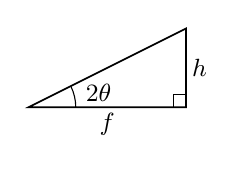
\begin{tikzpicture}[font=\small,baseline=(b)]
  \coordinate (b) at (0,0.4);
  \draw[line width=0.6pt] (0,0) -- (2.0,0) -- (2.0,1.0) -- cycle;
  \draw[line width=0.4pt] (2.0,0) ++(-0.16,0) -- ++(0,0.16) -- ++(0.16,0);
  \draw[line width=0.4pt] (0.6,0) arc[start angle=0,end angle={atan(1.0/2.0)},radius=0.6];
  \node[inner sep=0pt,anchor=base west] at (0.72,0.07) {$2\theta$};
  \node[anchor=north,inner sep=2pt] at (1.0,0) {$f$};
  \node[anchor=west,inner sep=2pt] at (2.0,0.5) {$h$};
\end{tikzpicture}
